\documentclass[french,12pt]{article}
\usepackage[T1]{fontenc}
\usepackage[utf8]{inputenc}
\usepackage{lmodern}
\usepackage[a4paper,top=1.0cm, left=1.0cm, right = 1.0cm, bottom = 1.2cm]{geometry}
\usepackage{amsmath}
\usepackage{tikz}
\usepackage{pgfplots}
\usepackage{subfig}

\def\spaceans{\underline{\hspace{1cm}}}
\def\spaceTF{$\big(\quad\big)$}

\usepackage{tikz}
\usepackage{physics}
\usepackage[outline]{contour} % glow around text
\usetikzlibrary{calc}
\usetikzlibrary{decorations.markings}
\usetikzlibrary{angles,quotes} % for pic
\usetikzlibrary{arrows.meta} % for arrow size
\usetikzlibrary{bending} % for arrow head angle
\usetikzlibrary{decorations.pathmorphing} % for decorate random steps
\tikzset{>=latex} % for LaTeX arrow head
\usepackage{xcolor}
\contourlength{1.3pt}

\colorlet{xcol}{blue!70!black}
\colorlet{xcol'}{xcol!50!red}
\colorlet{vcol}{green!45!black}
\colorlet{acol}{red!50!blue!80!black!80}
\tikzstyle{rvec}=[->,very thick,xcol,line cap=round]
\tikzstyle{vvec}=[->,very thick,vcol,line cap=round]
\tikzstyle{avec}=[->,very thick,acol,line cap=round]
\colorlet{myred}{red!65!black}
\tikzstyle{force}=[->,myred,very thick,line cap=round]
\tikzstyle{mass}=[line width=0.5,draw=red!50!black,fill=red!50!black!10,rounded corners=1,
top color=red!50!black!30,bottom color=red!50!black!10,shading angle=20]
\tikzstyle{disk}=[line width=0.5,orange!30!black,fill=orange!40!black!10,
top color=orange!40!black!20,bottom color=orange!40!black!10,shading angle=20]
\tikzstyle{pole}=[line width=0.5,blue!20!black,fill=orange!20!black!10,
top color=blue!20!black!20,bottom color=blue!20!black!10,shading angle=20]
\tikzstyle{rope}=[brown!70!black,line width=1,line cap=round] %very thick
\tikzstyle{myarr}=[-{Latex[length=3,width=2,flex'=1]},thin]
\tikzstyle{mydashed}=[dash pattern=on 2pt off 1pt]
\def\rope#1{ \draw[rope,black,line width=1.4] #1; \draw[rope,line width=1.1] #1; }
\def\tick#1#2{\draw[thick] (#1) ++ (#2:0.1) --++ (#2-180:0.2)}
\newcommand\rightAngle[4]{
	\pgfmathanglebetweenpoints{\pgfpointanchor{#2}{center}}{\pgfpointanchor{#3}{center}}
	\coordinate (tmpRA) at ($(#2)+(\pgfmathresult+45:#4)$);
	%\draw[white,line width=0.6] ($(#2)!(tmpRA)!(#1)$) -- (tmpRA) -- ($(#2)!(tmpRA)!(#3)$);
	\draw[black] ($(#2)!(tmpRA)!(#1)$) -- (tmpRA) -- ($(#2)!(tmpRA)!(#3)$);
}

\def\L{3.1}     % axis lengths
\def\R{1.0*\L}  % position vector radial distance
\def\Rang{52}   % position vector angle
\def\ang{25}    % angle of the CM velocity


\begin{document}
Responsable TD: Felipe FIGUEREDO ROCHA, \texttt{felipe.figueredo-rocha@u-pec.fr} \\
Obs1: Ces questions peuvent contenir des imprécisions, merci de se repérer au TD pour peut-être clarifier vous-même quelques imprécisions. \\
Obs2: Merci de signalez des imprécisions sur l'email ci-dessus. \\ 
Obs3: Des question extrêmement importants pour CC2 sont marqués avec {(\bf CC2)}. Celles extrêmement importants pour l'examen mais qui ne sont pas important pour CC2 sont dénotés {(\bf E)}. Les questions qui sont plutôt des outils à des questions de du CC2 ou Examen, sont marquées en {(\bf G)}.
\section*{Rappels de maths}
\begin{enumerate}

\item {(\bf G)} En utilisant $\cos(a \pm b) = \cos a \cos b \mp \sin a \sin b$ et $\sin(a \pm b) = \sin a \cos b \pm \cos a \sin b$, vérifiez que $\cos(\frac{\pi}{2} - \theta) = \sin \theta$, $\sin(\frac{\pi}{2} - \theta) = \cos \theta$, $\cos(\pi - \theta) = -\cos \theta$. Puis, sans utiliser les formules, vérifiez ces résultats en utilisant le cercle trigonométrique.



\item {(\bf G)} Soit $\vec{u}$ et $\vec{w}$ vecteurs unitaires tels que $\vec{u} \perp \vec{w}$. Par définition du produit scalaire, la projection de $\vec{P}$ sur $\vec{u}$ est donné par $\vec{P} \cdot \vec{u} = \| \vec{P} \| \cos \theta_1$. Calculez les projections $\vec{P} \cdot \vec{w}$, $\vec{R} \cdot \vec{u}$ et $\vec{R} \cdot \vec{w}$ en fonction des angles $\theta_1$ et $\theta_2$ en utilisant la définition du produit scalaire (formule avec $\cos$, pas en composantes) et des relations du exercice 1 (attention! l'angle entre $\vec{R}$ et $\vec{u}$ n'est pas $\theta_2$ mais plutôt $\pi - \theta_2$) . Simplifiez au maximum vos résultats. Vérifiez ces calculs d'une façon géometrique/visuelle (comme nous faisons en TD) en utilisant directement les définitions de sinus et cosinus d'un triangle rectangle et en vérifiant si la projection est négatif ou positif.

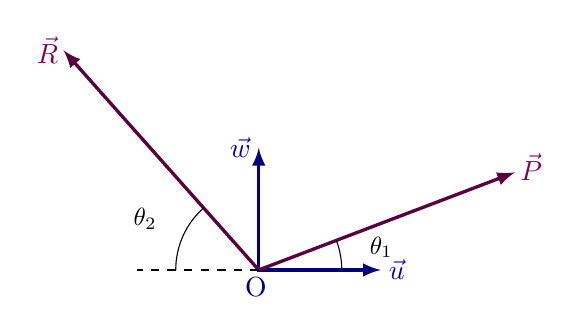
\begin{tikzpicture}
	\coordinate (O) at (0,0);
	\coordinate (X) at (0.5*\L,0);
	\coordinate (Y) at (0,0.5*\L);
	\coordinate (C) at (-0.5*\L,0);
	\coordinate (A) at (1.05*\L, 0.4*\L);
	\coordinate (B) at (-0.8*\L, 0.9*\L);
	
	% AXES
	\draw[<->,very thick,xcol!70!black]
	(X) node[right=-1,xcol] {$\vec{u}$} -- (O) node[left=1,below=-1] {O} --
	(Y) node[left=-1,xcol] {$\vec{w}$};
	\draw[<->,very thick,xcol'!70!black]
	(A) node[above=2,right=-2,xcol'] {$\Vec{P}$} -- (O) --
	(B) node[left=-2,xcol'] {$\Vec{R}$};
	
	\draw [dashed] (O) -- (C);	
	
	\draw pic["$\theta_1$"{scale=0.9},
	draw,angle radius=30,angle eccentricity=1.5] {angle=X--O--A};
	\draw pic["$\theta_2$"{scale=0.9},
	draw,angle radius=30,angle eccentricity=1.5] {angle=B--O--C};
\end{tikzpicture}


\item {(\bf G)} Soit $R(O, \vec{u}_x, \vec{u}_y)$ et $R^*(O, \vec{u}_x^*, \vec{u}_y^*)$ deux repères orthonormés. Pour définir $R^*$ on applique une rotation $\theta$ à $R$ dans le sens antihoraire (voir figure ci-dessous). D'abord, vérifiez que tout les distances de la figure sont corrects et puis montrez que
\begin{align} \label{eq:change_basis}
	\vec{OP} = x \vec{u}_x + y \vec{u}_y = (x \cos \theta + y \sin \theta) \vec{u}_x^* + (y \cos \theta - x \sin \theta) \vec{u}_y^*.
\end{align}

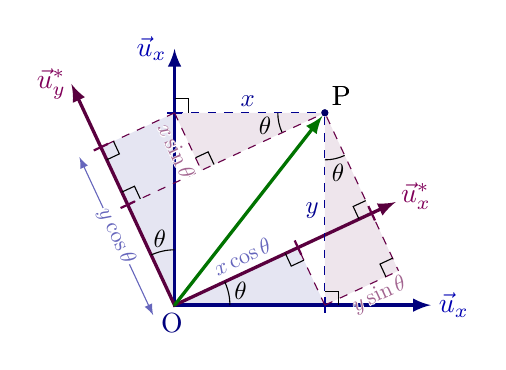
\begin{tikzpicture}
	\coordinate (O) at (0,0);
	\coordinate (X) at (1.05*\L,0);
	\coordinate (Y) at (0,1.05*\L);
	\coordinate (X') at (\ang:\L);
	\coordinate (Y') at (90+\ang:\L);
	\coordinate (R) at (\Rang:\R);
	\node[fill=blue!40!black,circle,inner sep=0.9] (R') at (R) {};
	\node[above right=-1] at (R') {P};
	\coordinate (Rx) at (0:{\R*cos(\Rang)});
	\coordinate (Ry) at (90:{\R*sin(\Rang)}); %($(Y)!(O)!(R)$);
	\coordinate (Rx') at (\ang:{\R*cos(\Rang-\ang)});
	\coordinate (Ry') at (90+\ang:{\R*sin(\Rang-\ang)});
	
	\coordinate (Rx'') at (\ang:{\R*cos(\Rang)*cos(\ang)});     % projection of Rx on x' axis
	\coordinate (Ry'') at (90+\ang:{\R*sin(\Rang)*cos(\ang)});  % projection of Ry on y' axis
	\coordinate (Rx''') at ($(R')+(-90+\ang:{\R*sin(\Rang)*cos(\ang)})$); % projection of Rx on R-Rx' line
	\coordinate (Ry''') at ($(R')+(180+\ang:{\R*cos(\Rang)*cos(\ang)})$); % projection of Ry on R-Ry' linex
	
	% TRIANGLES
	\fill[xcol!70!black!10]
	(O) -- (Rx) -- (Rx'') -- cycle
	(O) -- (Ry) -- (Ry'') -- cycle;
	\fill[xcol'!70!black!10]
	(R) -- (Rx) -- (Rx''') -- cycle
	(R) -- (Ry) -- (Ry''') -- cycle;
	\node[fill=blue!40!black,circle,inner sep=0.9] at (R') {};
	\node[above right=-1] at (R') {P};
	
	% AXES
	\draw[<->,very thick,xcol!70!black]
	(X) node[right=-1,xcol] {$\vec{u}_x$} -- (O) node[left=1,below=-1] {O} --
	(Y) node[left=-1,xcol] {$\vec{u}_x$};
	\draw[<->,very thick,xcol'!70!black]
	(X') node[above=2,right=-2,xcol'] {$\vec{u}_x^*$} -- (O) --
	(Y') node[left=-2,xcol'] {$\vec{u}_y^*$};
	
	% POSITION VECTOR
	\draw[vvec,line cap=round] (O) -- (R'); %node[midway,left=2,above=1] {$\vb{r}$};
	\draw pic["$\theta$"{scale=0.9},
	draw,angle radius=20,angle eccentricity=1.22] {angle=X--O--X'};
	\draw pic["$\theta$"{scale=0.9},
	draw,angle radius=20,angle eccentricity=1.22] {angle=Y--O--Y'};
	\draw pic["$\theta$"{scale=0.9},
	draw,angle radius=17,angle eccentricity=1.30] {angle=Rx--R'--Rx'};
	\draw pic["$\theta$"{scale=0.9},
	draw,angle radius=17,angle eccentricity=1.30] {angle=Ry--R'--Ry'};
	
	% ANGLES
	\begin{scope}[xcol!80!black]
		\draw[dashed]
		(Ry) -- (R') node[midway,above=-1,scale=0.9] {$x$} --
		(Rx) node[midway,left=-1,scale=0.9] {$y$};
		\tick{Rx}{90};
		\tick{Ry}{0};
		\rightAngle{R'}{Rx}{X}{0.25}
		\rightAngle{Y}{Ry}{R'}{0.25}
	\end{scope}
	\begin{scope}[xcol'!80!black]
		\draw[dashed] (Ry') -- (R') -- (Rx''');
		\draw[dashed] (Ry) -- (Ry'');
		\draw[dashed] (Rx) -- (Rx'');
		\draw[dashed] (Rx) -- (Rx''');
		\draw[dashed] (Ry) -- (Ry''');
		\tick{Rx'}{90+\ang};
		\tick{Ry'}{\ang};
		\tick{Rx''}{90+\ang};
		\tick{Ry''}{\ang};
		\rightAngle{X'}{Rx'}{R'}{0.25}
		\rightAngle{Y'}{Ry'}{R'}{0.25}
		\rightAngle{Rx}{Rx''}{O}{0.25}
		\rightAngle{Ry}{Ry''}{O}{0.25}
		\rightAngle{Ry}{Ry'''}{R}{0.25}
		\rightAngle{Rx}{Rx'''}{R}{0.25}
	\end{scope}
	
	% LENGTHS
	%\node[xcol!70!black,above,scale=0.8] at ($(Ry)!0.5!(R)$) {$x$};
	\node[xcol!80!black!60,above,scale=0.8,rotate=\ang] at ($(O)!0.6!(Rx'')$) {$x \cos\theta$};
	\node[xcol'!80!black!60,right=1,below=-2,scale=0.8,rotate=\ang] at ($(Rx)!0.6!(Rx''')$) {\contour{white}{$y\sin\theta$}};
	%\node[xcol!80!black!60,below=4,scale=0.8,rotate=-90+\ang] at ($(O)!0.6!(Ry'')$) {$y\cos\theta$};
	\node[xcol'!80!black!60,below=-1,scale=0.8,rotate=-90+\ang] at ($(Ry)!0.6!(Ry''')$) {\contour{white}{$x\sin\theta$}};
	\draw[<->,xcol!80!black!60]
	([shift={(180+\ang:0.3)}]O) -- ([shift={(180+\ang:0.3)}]Ry'')
	node[xcol!80!black!60,midway,scale=0.8,rotate=-90+\ang,fill=white,inner sep=0.5] {$y\cos\theta$};
	
\end{tikzpicture}
\item {(\bf G)} Tracer la fonction $x(t) = 2 \cos 2\pi t$ en $t\in[0 s, 2 s]$. Combien de fois la fonction si répète dans cette intervale? 
\item {(\bf G)} Tracer la fonction $x(t) = 3 \sin 4\pi t$ en $t\in[0 s, 1 s]$. Combien de fois la fonction si répète dans cette intervale? 
\item {(\bf G)} En définissant $T$ (on appelle de \textit{période} ce valeur) étant le temps nécessaire pour une fonction périodique  revenir a sa position dans un instant $t$ donné, c'est-à-dire $g(t + T) = g(t)$. Calculez $T$ pour les cas précédents (il faut juste diviser la taille d'intervale par le nombre de répétitions).
\item {(\bf G)} Pour une fonction périodique $x(t) = A \cos \omega t$ (pareil pour sinus), avec $A>0 {\rm \, m}, \omega > 0 {\rm \, rad/s}$, qu'est-ce que si passe avec $T$ (augment ou diminue) si i) $\omega$ augmente, ii) $\omega$ diminue. Le comportement de $T$ par rapport $\omega$ est proportionnelle ou inversement proportionnelle? 

\end{enumerate}

\section*{Questions à réfléchir pour le CC2 et examen}
\begin{enumerate}

\item {(\bf CC2)} Refaire 6) (rappel maths) en utilisant la formule $T = 2\pi/\omega$, où $\omega = 2 \pi {\rm rad/s}$ pour 1) et $\omega = 4 \pi {\rm rad/s}$ pour 2). Les résultats sont-ils identiques?

\item  {(\bf CC2)} Dans l'exercise du pendule (Ex 10 du TD), notez que la projection de la force poids $\vec{P}$ dans le repère polaire n'est qu'une application de la formule \eqref{eq:change_basis}, pour le cas spécifique $\vec{u}_x^* = \vec{u}_r, \vec{u}_y^* = \vec{u}_{\theta}$ et $\vec{P} = mg \vec{u}_x$ (justifiez-les). Calculez $\vec{P}$ en repère polaire et comparez avec les résultats obtenus en TD.


\item {(\bf CC2)} Etant donné l'équation différentiel du pendule (ex 10.7), on a étudié la solution $\theta(t) = \theta_0 \cos \omega t$, qui est valable pour les conditions initiales $\theta(0) = \theta_0$ et $\dot{\theta}(0) = 0$ (ex 10.8). Imaginez maintenant qu'on change les conditions initiales pour $\theta(0) = 0$ et $\dot{\theta}(0) = \omega_0$.
\begin{enumerate}
\item Est-ce que la solution $\theta(t) = \theta_0 \cos \omega t$ est encore valable?
\item Vérifiez que la solution du type $\theta(t) = A \sin \omega t$ peut satisfaire l'équation différentiel et les nouvelles condition initiales. Quel est la valeur pour $A$ en fonction des conditions initiales? 
\item {(\bf G)} Dans le cas général $\theta(0) = \theta_0$ et $\dot{\theta}(0) = \omega_0$, vérifiez qu'une solution du type $\theta(t) = A \sin \omega t + B \cos \omega t$ est solution de l'équation différentiel en satisfaisant les nouvelles conditions initiales (trouvez les valeurs $A$ et $B$. 

\end{enumerate}

\item {(\bf E)} Dessinez un plan incliné d'hauteur $H$ et angle $\theta$ avec l'horizontale et placez une particule de masse $m$ au sommet de ce plan incliné (accélération de pesanteur vers le bas). Proposez un repère que soit adapté à analyse de ce mouvement par le PFD (origine + base orthonormé). Écrivez donc les équations de PFD dans la cas où il n'y a pas de frottement et dans le cas ou le frottement est une constant donné $f$. Si la particule est largué du sommet avec vitesse nulle, trouvez la vitesse de ce particule en arrivant au sol par la méthode PFD dans les deux cas (après avoir trouver les expressions analytiques, vous pouvez remplacez quelques variables par des valeurs numériques pour vous convaincre que la vitesse dans le cas où le frottement est actif est plus petit que dans le cas sans frottement). Serait-il possible de calculer cette vitesse finale avec le théorème d'énergie cinétique? et la réaction normale à ce plan?

\item {(\bf CC2)} La force élastique d'un ressort horizontale est donné par $\vec{f}_{el} = -k x \vec{u}_x$ (pour simplifier on considère que l'origine du repère est placé sur la position d'équilibre du ressort). Montrez que le travail effectué par ce ressort entre la position $x=x_A$ initiale et la position $x=x_B$ finale est donné par 
$$
W_{A\to B}(\vec{f}_{el}) = \frac{k}{2}(x_A^2 - x_B^2).
$$
En compression ($x_A<0$ et $x_B<0$), quel est la condition pour le travail soit positif. En traction ($x_A>0$ et $x_B>0$), quel est la condition pour le travail soit positif.

\item {(\bf CC2)} Une particule de masse $m$ tombe en chute libre verticalement et touche avec vitesse $\vec{v}_0 = v_0 \vec{u}_y$ ($\vec{u}_y$ pointe le bas) un ressort verticale (négligez la longueur d'équilibre du ressort). En utilisant le théorème d'énergie cinétique, calculez la compression du ressort nécessaire a freiner la particule jusqu'à vitesse nulle (conseil: pendant la compression il y deux travails au même temps: de la force élastique et de la force poids donné par $\vec{P} = m g \vec{u}_y $ vers le bas).

\item {(\bf G)} Quel est la différence entre référentiel et repère ? (voir notes de cours, article wikipedia: cherchez référentiel (physique), etc)
\item {(\bf E)} Ennoncer le PFD en équations et en mots (en référentiel galiléan ou inertiel). 
\item {(\bf E)} Ennoncer le Theorème d'énergie cinétique en équations et en mots (en référentiel galiléan ou inertiel).
\item {(\bf G)} Pourquoi dans les exercices du pendule, on a pu utilisé le PFD et le Théorème d'énergie cinétique dans sa forme classique (en référentiel galiléan ou inertiel), même en utilisant un repère polaire (qui est mobile)?  
\item {(\bf CC2, E)} Un mouvement circulaire avec $\ddot{\theta}(t) = 0$ est-il dit uniforme? qu'est-ce que si passe avec $\Vec{a}(t)$, est-il nulle?
\item {(\bf CC2, E)} Sachant que $\Vec{v}(t) = R\dot{\theta} \Vec{u}_{\theta}$, $\Vec{a}(t) = - \dot{\theta} R \Vec{u}_r$ (démontrez-les si vous voulez) pour le mouvement circulaire uniforme, dessinez ces vecteurs pour une position de la particule librement choisi.
\item {(\bf CC2, E)} Sachant que $\Vec{v}(t) = R\dot{\theta} \Vec{u}_{\theta}$, $\Vec{a}(t) = - \dot{\theta} R \Vec{u}_r + \ddot{\theta} R \Vec{u}_{\theta}$ (démontrez-les si vous voulez) pour le mouvement circulaire non uniforme, dessinez ces vecteurs pour une position de la particule librement choisi. Seriez-vous capable de savoir si le mouvement est circulaire uniforme ou non uniforme juste avec le dessin de vecteur acceleration. 
\item {(\bf E)} Quel-est la condition (cinématique) nécessaire pour que un mouvement soit du type rectiligne uniforme (notez que le mot uniforme est employé dans sens différent dans l'exercise 12))? 
 
\item {(\bf G)} Etant donné $\theta(t) = \omega t$ ($\omega >0$) et $r(\theta(t)) = A + B \theta(t)$ ($A>0, B>0$), décrivant le mouvement d'une particule, calculez le vecteur vitesse et acceleration en repère polaire (utilisez les formules générales écrits dans le rappel du TD). Peut-on dire que cette la trajectoire dessine une spirale dans le plan $x \times y$ (utilisez $x(t) = r(\theta(t)) \cos \theta(t), y(t) =  r(\theta(t)) \sin \theta(t)$ pour aider dans votre raisonement)? 

% ANGLED ACCELERATION - opposite

% ROTATION + angles

\end{enumerate}

%\begin{tikzpicture}
%	\coordinate (O) at (0,0);
%	\coordinate (X) at (1.05*\L,0);
%	\coordinate (Y) at (0,1.05*\L);
%	\coordinate (X') at (\ang:\L);
%	\coordinate (Y') at (90+\ang:\L);
%	\coordinate (R) at (\Rang:\R);
%	\node[fill=blue!40!black,circle,inner sep=0.9] (R') at (R) {};
%	\node[above right=-1] at (R') {P};
%	\coordinate (Rx) at (0:{\R*cos(\Rang)});
%	\coordinate (Ry) at (90:{\R*sin(\Rang)}); %($(Y)!(O)!(R)$);
%	\coordinate (Rx') at (\ang:{\R*cos(\Rang-\ang)});
%	\coordinate (Ry') at (90+\ang:{\R*sin(\Rang-\ang)});
%	
%	% AXES
%	\draw[<->,very thick,xcol!70!black]
%	(X) node[right=-1,xcol] {$x$} -- (O) node[below left=-3] {O} --
%	(Y) node[left=-1,xcol] {$y$};
%	\draw[<->,very thick,xcol'!70!black]
%	(X') node[above=2,right=-2,xcol'] {$x'$} -- (O) --
%	(Y') node[left=-2,xcol'] {$y'$};
%	
%	% POSITION VECTOR
%	\draw[rvec,vvec,line cap=round] (O) -- (R') node[midway,left=2,above=1] {$\vb{r}$};
%	\draw pic[-{Latex[length=3,width=2,flex'=1]},"$\theta=\omega t$"{scale=0.95,above=2,right},
%	draw,angle radius=20,angle eccentricity=1] {angle=X--O--X'};
%	
%	% ANGLES
%	\begin{scope}[xcol!70!black]
%		\draw[dashed] (Ry) -- (R') -- (Rx);
%		\tick{Rx}{90};
%		\tick{Ry}{0};
%		\rightAngle{R'}{Rx}{X}{0.25}
%		\rightAngle{Y}{Ry}{R'}{0.25}
%	\end{scope}
%	\begin{scope}[xcol'!70!black]
%		\draw[dashed] (Ry') -- (R') -- (Rx');
%		\tick{Rx'}{90+\ang};
%		\tick{Ry'}{\ang};
%		\rightAngle{X'}{Rx'}{R'}{0.25}
%		\rightAngle{Y'}{Ry'}{R'}{0.25}
%	\end{scope}
%	
%\end{tikzpicture}




\end{document}
